\documentclass{beamer}

% Préambule - Inclusion de packages, définitions de thèmes, etc.
\usepackage[french]{babel} % Langue
\usepackage[utf8]{inputenc} % Encodage des caractères
\usepackage[T1]{fontenc} % Encodage des polices
\usepackage{tikz}
\usetikzlibrary{quantikz}


% Thème de la présentation
\usetheme{Frankfurt} % Vous pouvez changer le thème ici

% Définir des couleurs personnalisées
\definecolor{maCouleurPrincipale}{RGB}{0, 102, 204} % Définir une couleur personnalisée
\setbeamercolor{structure}{fg=maCouleurPrincipale} % Utiliser la couleur personnalisée pour la structure principale
\setbeamercolor{title}{bg=maCouleurPrincipale, fg=white} % Couleurs pour le titre


% Informations de la première page
\title{Calcul Quantique Adiabatique}
\author{Côme Périn - Sam Gubernator}
\institute{ENSEIRB-MATMECA}
\date{Décembre 2023} % Date de la présentation

\begin{document}

% Diapositive du titre
\begin{frame}
\titlepage
\end{frame}

% Diapositive de la table des matières
\begin{frame}
\frametitle{Sommaire}
\tableofcontents
\end{frame}

\section{Outils de compréhension}
\begin{frame}{Calcul basé sur le circuit}
% Exemple de porte quantique, etc.

On considère un problème. \\
On construit un circuit quantique pour y répondre.

\begin{center}
\begin{quantikz}
\ket{0} &\gate{H}&\gate[2]{U}& \meter{} \\
\ket{0} & \qw &&\qw
\end{quantikz}
\end{center}

Le système dans un état initial $\ket{\Psi_0}$ est modifié par des portes quantiques. Il finit dans l'état $\ket{\Psi_f}$. \medskip

Le système est modifié par des portes quantiques. \medskip

Une mesure finale répond au problème.

\end{frame}

\begin{frame}{Calcul quantique}
% Expliquer que la configuration d'un système est donnée par la hamiltonien
% Dire que le temps d"évolution est important

Équation de Schrödinger :
\begin{equation*}
    i\hbar\frac{d|\Psi(t) \rangle}{dt} = \hat{H}|\Psi(t)\rangle
\end{equation*}

\begin{itemize}
    \item La configuration du système (Énergie) est donnée par $\hat{H}$.
    \item Le calcul revient à faire évoluer H pendant un temps $\tau$.
    \item $\tau$ est le temps de calcul.
\end{itemize}

\end{frame}

% Section 2


\begin{frame}{Niveaux d'Énergie}
% Expliquer 
\begin{figure}
    \centering
    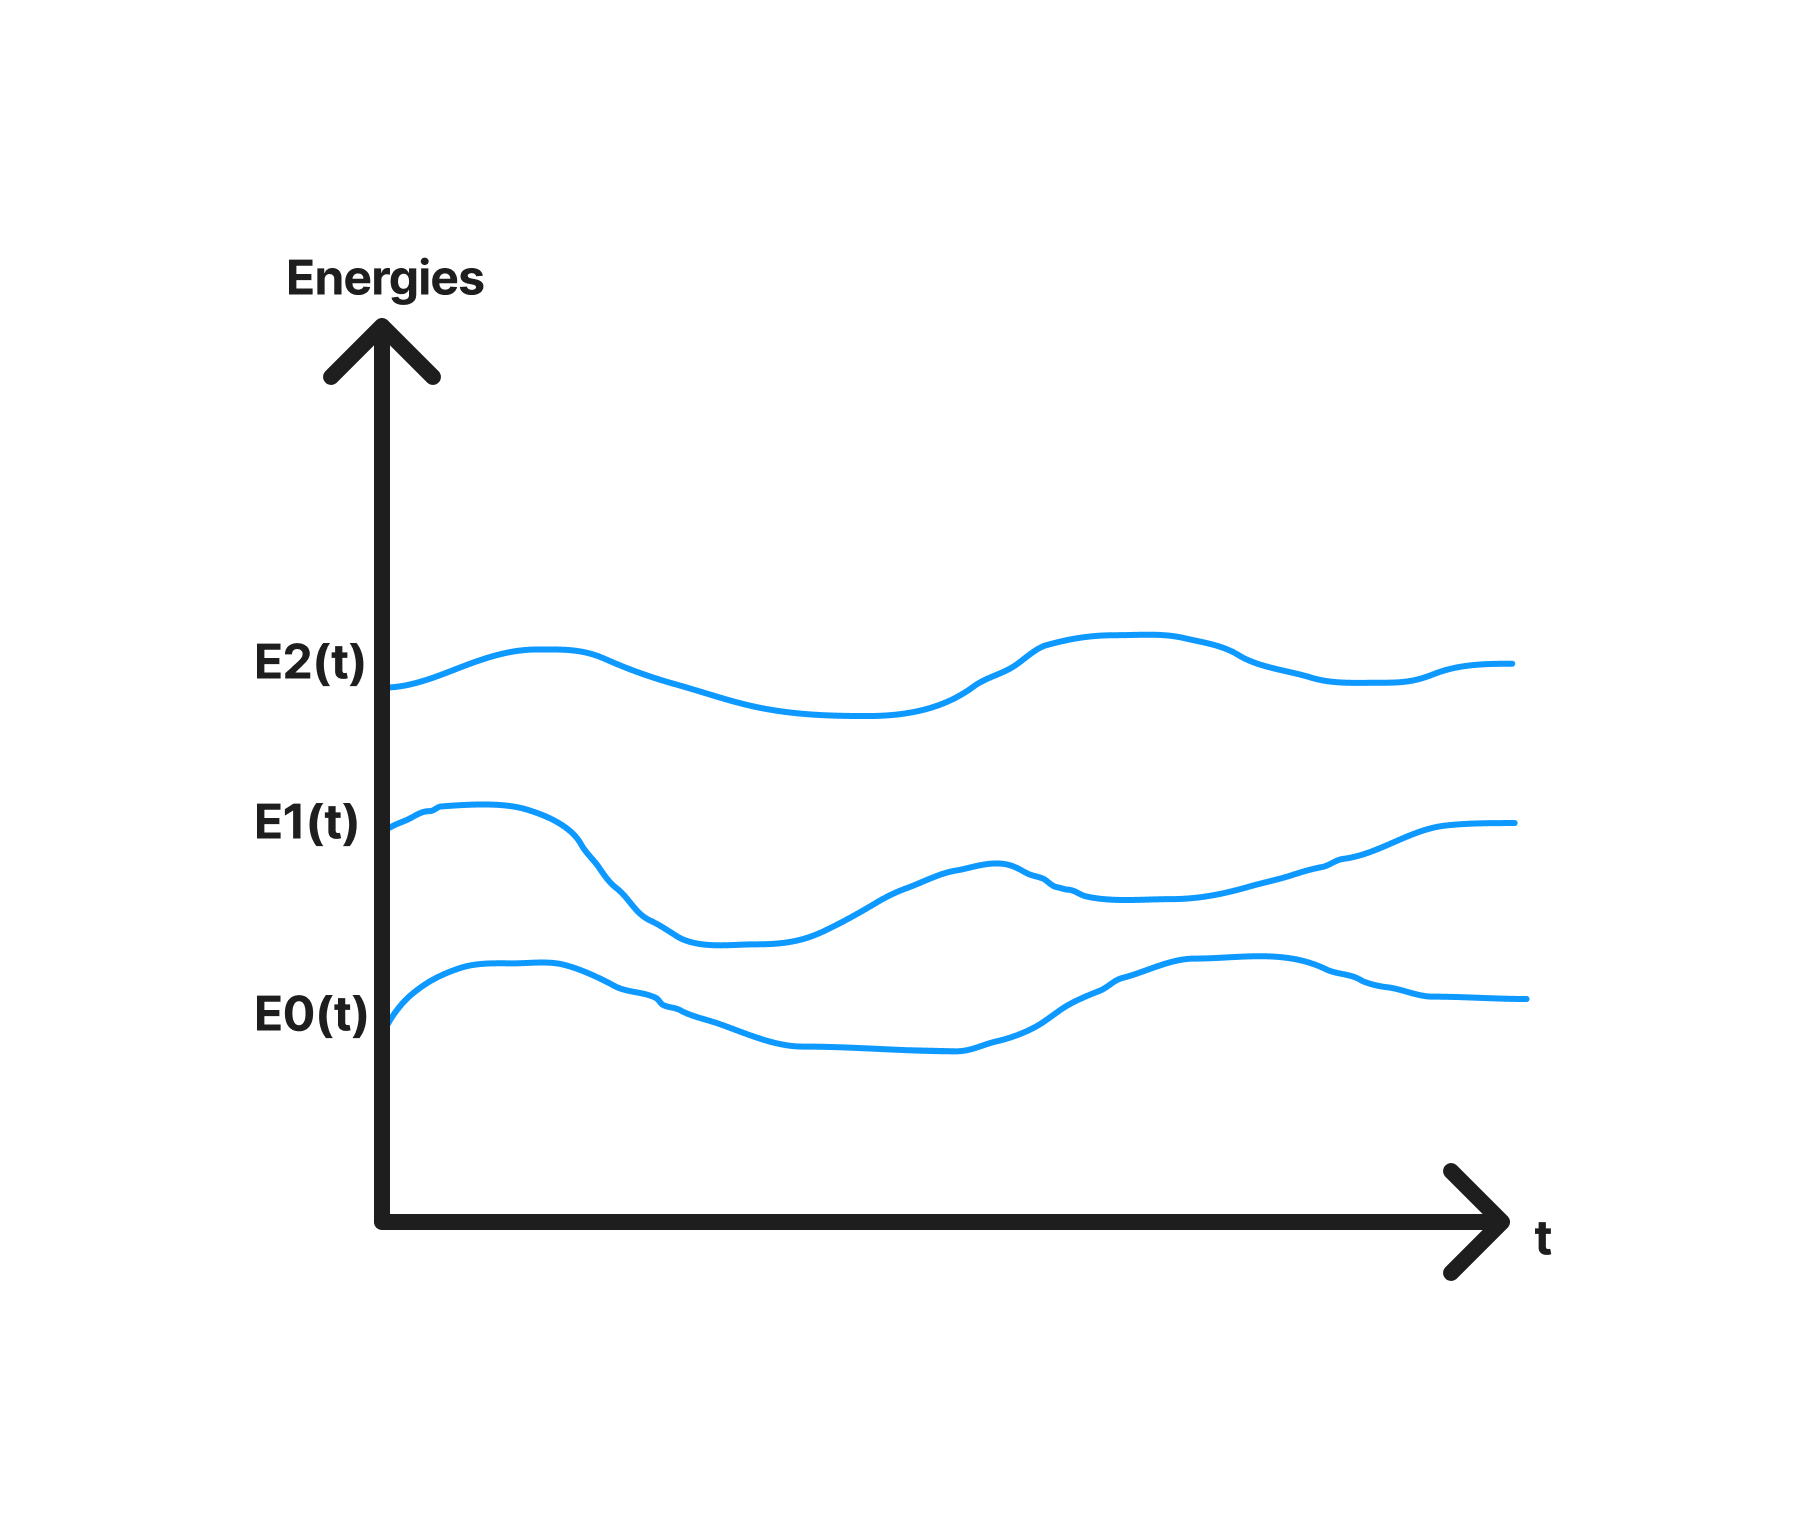
\includegraphics[scale=0.2]{rsc/energies.png}
    \caption{Évolution des niveaux d'énergie en fonction du temps}
    \label{fig:energie}
\end{figure}

\end{frame}

\begin{frame}{État propre}
    \centering
    1 niveau d'énergie, $\Leftrightarrow$ 1 état propre. 
\medskip

$$\forall t \in [t_0, t_f], H(t)\Psi_i(t) = E_i(t)\Psi_i(t)$$
\end{frame}

\begin{frame}{Processus adiabatique}
% Expliquer
% différent de l'adiabaticité en thermo

\begin{itemize}
    \item Différent de l'adiabaticité thermodynamique
    \item Plutôt analogue à une transformation statique en thermodynamique.
    \item Système soumis à une évolution lente de l'environnement ($\tau \xrightarrow{} \infty$)
\end{itemize}

\end{frame}

\section{Fonctionnement}
\begin{frame}{Théorème adiabatique}
    \begin{itemize}
        \item Processus adiabatique
        \item Niveau d'énergie initial suffisamment isolé 
    \end{itemize}

    Dans ce cas, la fonction d'onde finale $\Psi_f$ partage la même forme fonctionnelle que la fonction d'onde initiale $\Psi_0$. \medskip

    Autrement dit : on reste sur le même état propre/niveau d'énergie.

\end{frame}


% Section 3
\begin{frame}{Calcul quantique adiabatique}
% Contenu de la diapositive
\textbf{Objectif} : résoudre un problème complexe. 

\medskip

On détermine $H_f$ un hamiltonien complexe de sorte que son état fondamental décrive une solution du problème. 

\medskip

\textbf{Conditions initiales :} L'hamiltonien initial du système $H_0$ est simple. On place le système dans son état fondamental.

\medskip

\textbf{Calcul :} On fait évoluer adiabatiquement $H_0$ vers $H_f$, la mesure finale de $\Psi_f$ donne la solution optimale au problème complexe.

\end{frame}

\section{Utilisation de la méthode}
\begin{frame}{Exemple de résolution}
    \begin{figure}
        \centering
        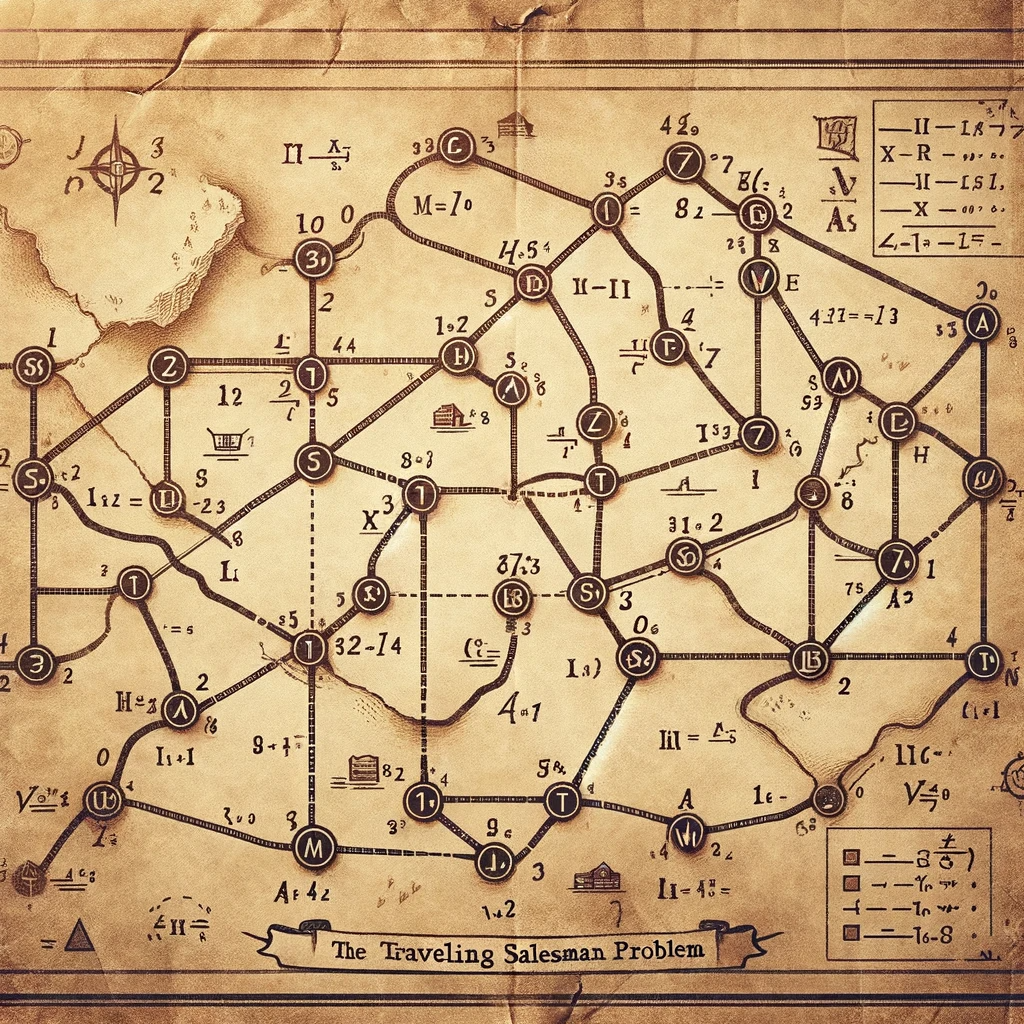
\includegraphics[scale=0.1]{rsc/voy.png}
        \label{fig:salesman}
    \end{figure}

Des problèmes tels que celui du voyageur peuvent être transposé dans le monde physique et ainsi résolus par la méthode du calcul quantique adiabatique.
\end{frame}

\begin{frame}{Avantages et inconvénients}
    \begin{itemize}
        \item + Résolutions de problème complexes sans mesures intermédiaires
        \item + Assurance de trouver une solution optimale si adiabaticité conservée
        \item - Mise en pratique compliquée (bascule)
        \item - Vitesse d'exécution
    \end{itemize}
\end{frame}

% Diapositive des remerciements ou des questions
\begin{frame}
\Huge{\centerline{Merci pour votre attention}}
\Large{\centerline{Des questions ?}}
\end{frame}

\end{document}
